\documentclass[12pt,a4paper]{article}

\usepackage[utf8]{inputenc}
\usepackage[T1]{fontenc}
\usepackage[margin=2.5cm]{geometry}
\usepackage{amsmath, amssymb}
\usepackage{xcolor}
\usepackage{tikz}
\usepackage{booktabs}
\usepackage{listings}

\usetikzlibrary{shapes.geometric, arrows.meta, positioning, shapes.misc}

\definecolor{loadcolor}{HTML}{FF5722}
\definecolor{soilcolor}{HTML}{8D6E63}
\definecolor{pilecolor}{HTML}{2196F3}
\definecolor{fusioncolor}{HTML}{9C27B0}

\lstset{
  basicstyle=\ttfamily\small,
  keywordstyle=\color{blue!80!black}\bfseries,
  commentstyle=\color{green!50!black}\itshape,
  stringstyle=\color{red!70!black},
  backgroundcolor=\color{gray!8},
  frame=single, framerule=0.4pt,
  language=Python
}

\title{\textbf{Thermodynamic 21-Slot Model}\\[0.3em]
\large Load-Driven Soil Degradation with Physics Constraints}
\author{PFE Research Notes}
\date{March 2026}

\begin{document}
\maketitle

% ===========================================================
\section{Physics Principle from Sketch}
% ===========================================================

The hand-sketch prescribes:
\begin{align}
  S_1 &= \{G_0, H, e\}  \quad \text{(initial state: modulus, horizontal load, porosity)}  \\
  S_2 - S_1 &= 4 H_i [j]_{n=1}  \quad \text{(state change from load history)}
\end{align}

Key observations:
\begin{itemize}
  \item \textbf{Horizontal force H} and \textbf{Moment M} drive degradation
  \item \textbf{Stiffness C} decreases monotonically as load increases
  \item \textbf{Shear modulus ratio} $G/G_0 \to 0$ as cyclic strain accumulates
  \item \textbf{Thermodynamic constraint}: Energy dissipation and entropy always increase (2nd law)
  \item \textbf{Primary output}: $G/G_{\max}$ (soil shear modulus degradation)
\end{itemize}

Hardin--Drnevich degradation law (1972):
\[
  \frac{G}{G_0} = \frac{1}{1 + \left(\frac{\gamma}{\gamma_{\text{ref}}}\right)^{\alpha}}
\]
where $\gamma$ is cyclic strain, $\gamma_{\text{ref}}$ is reference strain, $\alpha \approx 0.9$.

% ===========================================================
\section{21-Slot Architecture}
% ===========================================================

\subsection{Organizational Structure}

\begin{figure}[h]
\centering
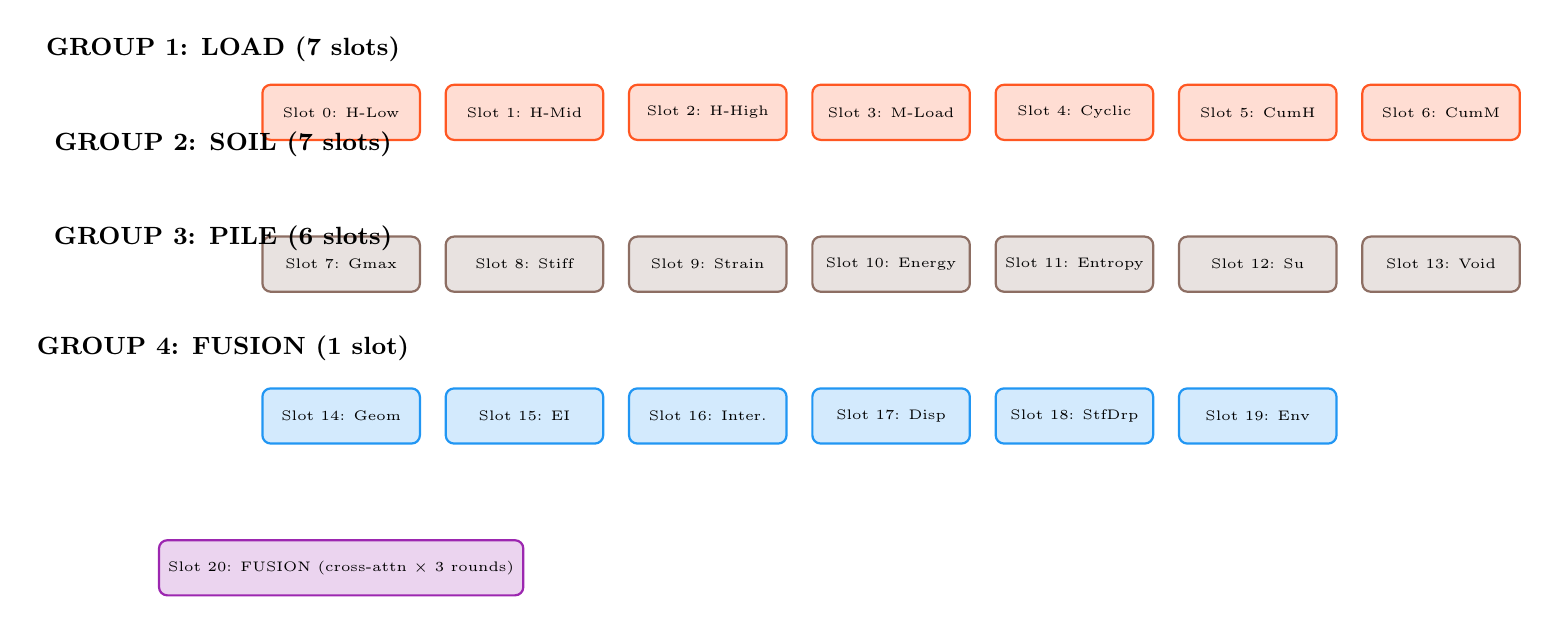
\begin{tikzpicture}[node distance=1cm, 
  slot/.style={rectangle, rounded corners=3pt, draw, thick, minimum width=2cm, minimum height=0.7cm, text centered, font=\tiny}]

  % Load slots
  \node[slot, fill=loadcolor!20, draw=loadcolor] (L1) {Slot 0: H-Low};
  \node[slot, fill=loadcolor!20, draw=loadcolor, right=0.3cm of L1] (L2) {Slot 1: H-Mid};
  \node[slot, fill=loadcolor!20, draw=loadcolor, right=0.3cm of L2] (L3) {Slot 2: H-High};
  \node[slot, fill=loadcolor!20, draw=loadcolor, right=0.3cm of L3] (L4) {Slot 3: M-Load};
  \node[slot, fill=loadcolor!20, draw=loadcolor, right=0.3cm of L4] (L5) {Slot 4: Cyclic};
  \node[slot, fill=loadcolor!20, draw=loadcolor, right=0.3cm of L5] (L6) {Slot 5: CumH};
  \node[slot, fill=loadcolor!20, draw=loadcolor, right=0.3cm of L6] (L7) {Slot 6: CumM};
  
  \node at (-1.5, 0.8) {\small \textbf{GROUP 1: LOAD (7 slots)}};
  
  % Soil slots
  \node[slot, fill=soilcolor!20, draw=soilcolor, below=1.2cm of L1] (S1) {Slot 7: Gmax};
  \node[slot, fill=soilcolor!20, draw=soilcolor, right=0.3cm of S1] (S2) {Slot 8: Stiff};
  \node[slot, fill=soilcolor!20, draw=soilcolor, right=0.3cm of S2] (S3) {Slot 9: Strain};
  \node[slot, fill=soilcolor!20, draw=soilcolor, right=0.3cm of S3] (S4) {Slot 10: Energy};
  \node[slot, fill=soilcolor!20, draw=soilcolor, right=0.3cm of S4] (S5) {Slot 11: Entropy};
  \node[slot, fill=soilcolor!20, draw=soilcolor, right=0.3cm of S5] (S6) {Slot 12: Su};
  \node[slot, fill=soilcolor!20, draw=soilcolor, right=0.3cm of S6] (S7) {Slot 13: Void};
  
  \node at (-1.5, -0.4) {\small \textbf{GROUP 2: SOIL (7 slots)}};
  
  % Pile slots
  \node[slot, fill=pilecolor!20, draw=pilecolor, below=1.2cm of S1] (P1) {Slot 14: Geom};
  \node[slot, fill=pilecolor!20, draw=pilecolor, right=0.3cm of P1] (P2) {Slot 15: EI};
  \node[slot, fill=pilecolor!20, draw=pilecolor, right=0.3cm of P2] (P3) {Slot 16: Inter.};
  \node[slot, fill=pilecolor!20, draw=pilecolor, right=0.3cm of P3] (P4) {Slot 17: Disp};
  \node[slot, fill=pilecolor!20, draw=pilecolor, right=0.3cm of P4] (P5) {Slot 18: StfDrp};
  \node[slot, fill=pilecolor!20, draw=pilecolor, right=0.3cm of P5] (P6) {Slot 19: Env};
  
  \node at (-1.5, -1.6) {\small \textbf{GROUP 3: PILE (6 slots)}};
  
  % Fusion
  \node[slot, fill=fusioncolor!20, draw=fusioncolor, below=1.2cm of P1, minimum width=4cm] (F) {Slot 20: FUSION (cross-attn $\times$ 3 rounds)};
  
  \node at (-1.5, -3.0) {\small \textbf{GROUP 4: FUSION (1 slot)}};

\end{tikzpicture}
\caption{21-Slot organization by domain.}
\end{figure}

\subsection{Input Data}

\begin{itemize}
  \item \textbf{Load.csv} $(B,T,6)$: $H$, $M$, $N_{\text{cycles}}$, $\text{freq}$, $\gamma_H^{\text{cum}}$, $\gamma_M^{\text{cum}}$
  \item \textbf{Soil.csv} $(B,T,5)$: $G_0$, $S_u$, $e$, $OCR$, $\text{deg\_factor}$
  \item \textbf{Pile.csv} $(B,T,4)$: $L$, $D$, $EI$, $t_{\text{wall}}$
  \item \textbf{Environment.csv} $(B,T,3)$: $H_{\text{wave}}$, $V_{\text{wind}}$, $d_{\text{water}}$
\end{itemize}

\subsection{Processing Flow}

Each slot follows the pattern:
\begin{enumerate}
  \item \textbf{Embedding}: map raw features $\to$ $d_{\text{model}}=48$ dimensions
  \item \textbf{Self-attention}: attend over time steps (capture temporal patterns)
  \item \textbf{Yield activation}: apply smooth saturation (physics-informed nonlinearity)
\end{enumerate}

The 20 specialized slots' outputs are then fused via:
\begin{enumerate}
  \item A learnable ``fusion query'' asks: ``what matters across all domains?''
  \item Cross-attention weights all 20 slots
  \item GRU iteratively refines (3 rounds)
  \item System-level yield activation
\end{enumerate}

\subsection{Output Targets (Primary: $G/G_{\max}$)}

\begin{itemize}
  \item $\mathbf{G/G_{\max}}$ — soil shear modulus ratio $\in [0.1, 1.0]$ \quad \textbf{(WEIGHTED 2.0)}
  \item $C_{\text{ratio}}$ — stiffness ratio $\in [0.05, 1.0]$
  \item $E_{\text{dissipated}}$ — normalized energy loss $\in [0, 1]$
  \item $S_{\text{entropy}}$ — entropy change (2nd law, unbounded)
\end{itemize}

% ===========================================================
\section{Physics Constraints}
% ===========================================================

\subsection{Thermodynamic Laws}

\textbf{1st Law (Energy):}
\[
  \frac{dU}{dt} = \dot{W} - \dot{Q}
\]
Energy dissipation due to cyclic loading increases monotonically:
\[
  E_{\text{dissipated}} = 1 - \frac{G}{G_0} \geq 0
\]

\textbf{2nd Law (Entropy):}
\[
  \frac{dS}{dt} = \frac{\dot{Q}}{T} + \dot{S}_{\text{gen}} \geq 0
\]
Soil undergoes irreversible deformation; entropy increases:
\[
  S_{\text{change}} = -\ln\left(\frac{G}{G_0}\right) \geq 0
\]

\subsection{Hardin--Drnevich Model}

Cyclic shear strain $\gamma$ accumulates from load history:
\[
  \gamma_{\text{total}} = \gamma_H + \gamma_M \quad (\text{normalized by }G_0, L, EI)
\]

Degradation follows:
\[
  \frac{G}{G_0} = \frac{1}{1 + (\gamma / \gamma_{\text{ref}})^{0.9}}
\]

\subsection{Stiffness Drop}

Lateral stiffness decreases as accumulated strain increases:
\[
  C(t) = C_{\max} \cdot \frac{G(t)}{G_0} \cdot e^{-0.5 \gamma(t)} \quad (\text{exponential decay})
\]

When a slot ``detects'' load trigger (via yield activation), stiffness drops sharply.

% ===========================================================
\section{Implementation Notes}
% ===========================================================

\begin{lstlisting}[caption=Core loop structure]
# All 21 slots process their domains
load_outputs = [slot_H_low(load), slot_H_mid(load), ...]
soil_outputs = [slot_Gmax(soil), slot_stiff(soil), ...]
pile_outputs = [slot_pile_geom(pile), ...]

# Fusion combines all 20 (indices 0-19)
all_slots = load_outputs + soil_outputs + pile_outputs
fused, attn_weights = fusion_slot(all_slots)

# Encoder + output heads
encoded = transformer_encoder(fused)
G_Gmax = head_G_Gmax(concat[encoded, aggregated_slots])
C_ratio = head_C_ratio(concat[encoded, aggregated_slots])
E_diss  = head_E_diss(concat[encoded, aggregated_slots])
entropy = head_entropy(concat[encoded, aggregated_slots])
\end{lstlisting}

\textbf{Loss function} heavily weights $G/G_{\max}$ (coefficient 2.0):
\[
  \mathcal{L} = 2.0 \, \text{MSE}(G_p, G_t) + 0.5 \, \text{MSE}(C_p, C_t) + 0.3 \, \text{MSE}(E_p, E_t) + 0.2 \, \text{MSE}(S_p, S_t)
\]

% ===========================================================
\section{Comparison: 5-Slot vs 21-Slot}
% ===========================================================

\begin{table}[h]
\centering
\begin{tabular}{lll}
\toprule
\textbf{Aspect} & \textbf{5-Slot} & \textbf{21-Slot} \\
\midrule
Specialized slots & 4 (CSV domains) & 20 (finer granularity) \\
Load representation & One slot & 7 slots (H ranges, M, cyclic, cumulative) \\
Soil degradation & One slot & 7 slots (Gmax, stiffness, strain, energy, entropy) \\
Pile response & Implicit & 6 slots (geometry, EI, interaction, displacement, drop) \\
Fusion & One slot & One slot (same mechanism) \\
Total parameters & Lower & Higher (more expressiveness) \\
Primary output & 4 targets & 4 targets (but heavy weight on G/Gmax) \\
Physics enforcement & Smooth activation & Smooth + thermodynamic penalties \\
\bottomrule
\end{tabular}
\end{table}

% ===========================================================
\section{Expected Behavior}
% ===========================================================

\begin{figure}[h]
\centering
\begin{tikzpicture}
  \begin{scope}[scale=2]
    % Axes
    \draw[thick] (0, 0) -- (4, 0) node[right] {Load};
    \draw[thick] (0, 0) -- (0, 3) node[above] {$G/G_0$};
    
    % Hardin-Drnevich curve
    \draw[thick, soilcolor] (0, 2.8) -- (0.5, 2.75) -- (1, 2.5) -- (1.5, 1.8) -- (2, 1.0) -- (2.5, 0.5) -- (3, 0.2) -- (3.5, 0.15);
    
    % Annotations
    \node at (0.5, 2.8) [above, font=\small] {Elastic};
    \node at (2, 1.5) [below, font=\small] {Transition};
    \node at (3.2, 0.5) [below, font=\small] {Plastic};
    
    % Arrows showing stiffness drop
    \draw[->, thick, red] (1, 2.5) -- (1.1, 2.3);
    \draw[->, thick, red] (2, 1.0) -- (2.1, 0.8);
    \draw[->, thick, red] (3, 0.2) -- (3.1, 0.1);
    
    \node at (3.8, 0.7) [right, font=\tiny, color=red] {$C$ drops};
  \end{scope}
\end{tikzpicture}
\caption{Expected $G/G_{\max}$ vs Load curve (Hardin--Drnevich).}
\end{figure}

As load (H, M, cycles) increases:
\begin{itemize}
  \item $\gamma_{\text{total}}$ accumulates
  \item $G/G_0$ decreases smoothly (elastic → plastic transition)
  \item Stiffness $C$ drops (1st \& 2nd law penalty)
  \item Entropy $S$ increases (irreversibility)
  \item Energy dissipation $E$ increases
\end{itemize}

\end{document}
